% !TeX program = lualatex
\documentclass[9.5pt,a4paper,landscape]{article}
\usepackage[a4paper,landscape,margin=8mm]{geometry}
\usepackage{fontspec}
\usepackage{microtype}
\defaultfontfeatures{Ligatures=TeX}

\IfFontExistsTF{Inter}{
  \usepackage[sfdefault,tabular]{inter}
}{
  \IfFontExistsTF{Helvetica Neue}{
    \setmainfont{Helvetica Neue}
  }{
    \setmainfont{TeX Gyre Heros}
  }
}
\IfFontExistsTF{JetBrains Mono}{
  \setmonofont{JetBrains Mono}[Scale=0.88]
}{
  \setmonofont{Latin Modern Mono}[Scale=0.88]
}

\usepackage{xcolor}
\usepackage{array}
\usepackage{adjustbox}
\usepackage{tikz}
\usetikzlibrary{arrows.meta,calc,positioning}
\pagestyle{empty}
\setlength{\parindent}{0pt}

\definecolor{ink}{RGB}{25,35,55}
\definecolor{surface}{RGB}{245,248,252}
\definecolor{primary}{RGB}{0,82,155}
\definecolor{celofill}{RGB}{253,236,200}
\definecolor{celostroke}{RGB}{166,124,0}
\definecolor{basefill}{RGB}{218,235,255}
\definecolor{basestroke}{RGB}{0,82,155}
\definecolor{solfill}{RGB}{234,218,255}
\definecolor{solstroke}{RGB}{122,43,210}
\definecolor{ethfill}{RGB}{221,228,250}
\definecolor{ethstroke}{RGB}{67,85,187}
\definecolor{vnxfill}{RGB}{224,242,240}
\definecolor{vnxstroke}{RGB}{0,107,98}
\definecolor{profit}{RGB}{21,122,78}
\definecolor{profitbg}{RGB}{220,245,230}
\definecolor{badgeamber}{RGB}{252,238,186}
\definecolor{badgeambertext}{RGB}{168,44,0}

\newcommand{\statlabel}[1]{%
  {\addfontfeatures{LetterSpace=35}%
   \fontsize{6.5}{8}\selectfont\bfseries\textcolor{ink!55}{\MakeUppercase{#1}}}}

\newcommand{\badge}[3]{%
  \tikz[baseline=(b.base)]{
    \node[draw=#2!40, fill=#2, rounded corners=1mm, inner xsep=1.8mm, inner ysep=0.6mm] (b) {%
      {\fontsize{7}{8.5}\selectfont\bfseries\textcolor{#3}{\MakeUppercase{#1}}}};
  }}

% Per-panel flow columns (mm)
\def\FxA{0}
\def\FxB{15.5}
\def\FxC{29}
\def\FxD{42.5}
\def\FxE{56}
\def\FxR{66}

\tikzset{
  hub/.style={
    draw=#1, thick, rounded corners=2pt,
    minimum height=7mm, minimum width=13mm,
    align=center, font=\fontsize{6.5}{7.8}\selectfont\bfseries, inner sep=0pt,
  },
  hub/.default=ink,
  act/.style={
    draw=#1!55, fill=white, rounded corners=2pt,
    minimum height=7mm, minimum width=11mm,
    align=center, font=\fontsize{6.2}{7.5}\selectfont, inner sep=0pt,
  },
  act/.default=ink,
  recon/.style={
    draw=primary!55, fill=primary!6, dashed, thick,
    rounded corners=2pt, minimum width=14mm, minimum height=7mm,
    align=center, font=\fontsize{6}{7}\selectfont\bfseries,
    text=primary, inner sep=0.5pt,
  },
  rowlbl/.style={
    anchor=east, font=\fontsize{6.2}{7.5}\selectfont\bfseries, text=ink!65,
    minimum width=17mm, align=right,
  },
  arr/.style={-{Stealth[length=1.6mm]}, thick, draw=ink!50},
  topo/.style={
    draw=#1, thick, rounded corners=2.5pt,
    minimum height=9mm, minimum width=18mm,
    align=center, font=\fontsize{7}{8.5}\selectfont\bfseries, inner sep=1pt,
  },
  topoarr/.style={-{Stealth[length=2mm]}, line width=0.9pt, draw=ink!55},
  topodash/.style={-{Stealth[length=1.8mm]}, line width=0.8pt, dashed, draw=primary!65},
}

\begin{document}
\color{ink}

% ── Header ──
\noindent
\begin{tabular}{@{}>{\raggedright\arraybackslash}p{0.64\linewidth}@{\hspace{0.02\linewidth}}>{\raggedright\arraybackslash}p{0.33\linewidth}@{}}
\begin{minipage}[t]{\linewidth}
  {\fontsize{17}{19}\selectfont\bfseries\color{primary} VCHF Menace --- Executive Route Map}\\[1pt]
  {\fontsize{9}{11}\selectfont Dual-hub VCHF arbitrage: \textbf{Celo USDT} + \textbf{Base USDC} · Solana USDC · VNX Platform}\\[0.5pt]
  {\fontsize{7}{9}\selectfont\textcolor{ink!60}{10 directed routes · buy VCHF on buy chain, sell on sell chain · closed-loop return after every arb}}
\end{minipage}
&
\begin{minipage}[t]{\linewidth}
  \raggedleft
  \badge{10 routes}{profitbg}{profit}\hspace{1.2mm}%
  \badge{dual hub}{badgeamber}{badgeambertext}\\[2pt]
  {\fontsize{6.8}{8.5}\selectfont\textcolor{ink!50}{2026-06-20 · github.com/Giansensey007/vchf\_menace}}
\end{minipage}
\\
\end{tabular}

\vspace{1mm}
\noindent\rule{\linewidth}{0.3pt}
\vspace{1mm}

% ── KPI strip ──
\noindent
\renewcommand{\arraystretch}{1.12}
\begin{tabular}{@{}>{\centering\arraybackslash}p{0.19\linewidth}
                  >{\centering\arraybackslash}p{0.19\linewidth}
                  >{\centering\arraybackslash}p{0.19\linewidth}
                  >{\centering\arraybackslash}p{0.19\linewidth}
                  >{\centering\arraybackslash}p{0.19\linewidth}@{}}
  \fcolorbox{primary!25}{surface}{%
    \begin{minipage}[c][13mm][c]{0.92\linewidth}
      \statlabel{Trade size}\\[0.5pt]
      {\fontsize{9.5}{11}\selectfont\bfseries 200\,--\,2{,}000 VCHF}
    \end{minipage}} &
  \fcolorbox{primary!25}{surface}{%
    \begin{minipage}[c][13mm][c]{0.92\linewidth}
      \statlabel{Min profit}\\[0.5pt]
      {\fontsize{9.5}{11}\selectfont\bfseries\textcolor{profit}{$\geq$\$5.00}}
    \end{minipage}} &
  \fcolorbox{celostroke!35}{celofill!40}{%
    \begin{minipage}[c][13mm][c]{0.92\linewidth}
      \statlabel{Celo hub}\\[0.5pt]
      {\fontsize{9}{11}\selectfont\bfseries\textcolor{celostroke}{USDT}}\\[-1pt]
      {\fontsize{6.5}{8}\selectfont CeloSwap}
    \end{minipage}} &
  \fcolorbox{basestroke!35}{basefill!50}{%
    \begin{minipage}[c][13mm][c]{0.92\linewidth}
      \statlabel{Base hub}\\[0.5pt]
      {\fontsize{9}{11}\selectfont\bfseries\textcolor{basestroke}{USDC}}\\[-1pt]
      {\fontsize{6.5}{8}\selectfont KyberSwap}
    \end{minipage}} &
  \fcolorbox{vnxstroke!35}{vnxfill}{%
    \begin{minipage}[c][13mm][c]{0.92\linewidth}
      \statlabel{Platform min}\\[0.5pt]
      {\fontsize{9.5}{11}\selectfont\bfseries 30 VCHF}\\[-1pt]
      {\fontsize{6.5}{8}\selectfont 5 VCHF on-chain deposit}
    \end{minipage}} \\
\end{tabular}

\vspace{1.5mm}

% ── Dual-hub topology (full width) ──
\noindent\fcolorbox{ink!12}{surface}{%
\begin{minipage}{\dimexpr\linewidth-2\fboxsep-2\fboxrule\relax}
\vspace{1mm}
\centering
{\fontsize{8}{9.5}\selectfont\bfseries\color{primary} Dual-hub topology --- Celo USDT \& Base USDC side by side}\\[2mm]
\adjustbox{width=0.98\linewidth}{%
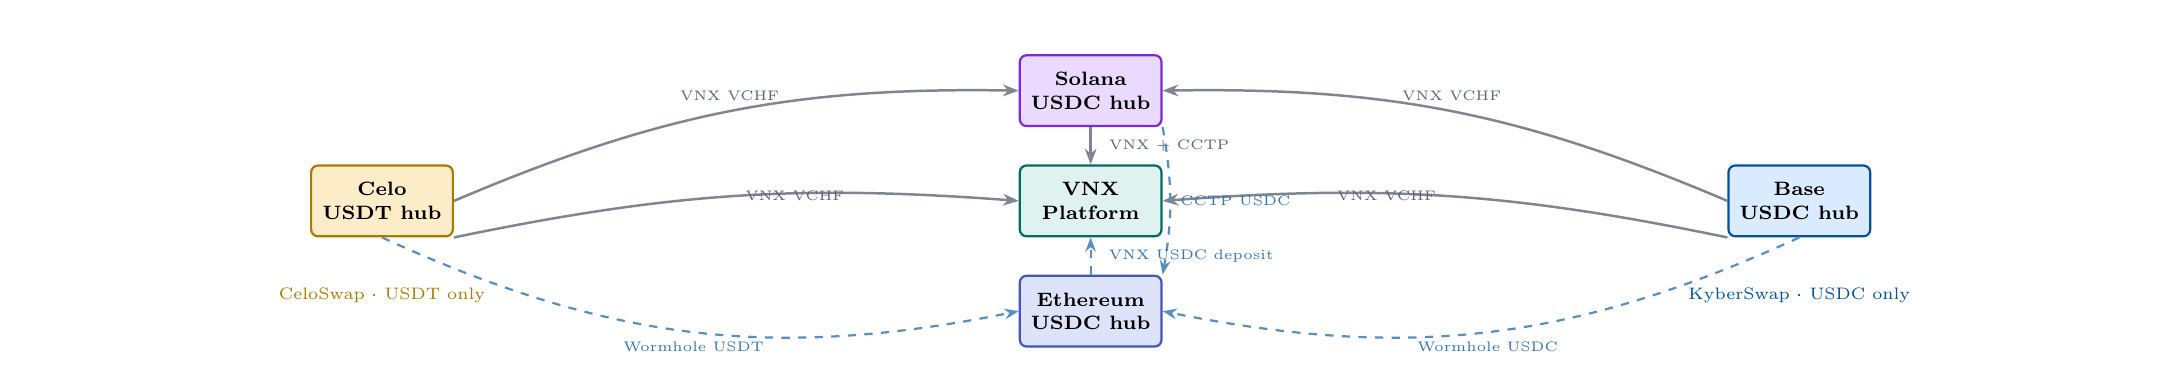
\begin{tikzpicture}[x=1mm,y=-1mm]
  \useasboundingbox (0,0) rectangle (270,42);

  % Hub nodes
  \node[topo=celostroke, fill=celofill] (celo) at (45,22) {Celo\\USDT hub};
  \node[topo=basestroke, fill=basefill] (base) at (225,22) {Base\\USDC hub};
  \node[topo=solstroke, fill=solfill] (sol) at (135,8) {Solana\\USDC hub};
  \node[topo=vnxstroke, fill=vnxfill] (vnx) at (135,22) {VNX\\Platform};
  \node[topo=ethstroke, fill=ethfill] (eth) at (135,36) {Ethereum\\USDC hub};

  % VNX VCHF bridges (solid)
  \draw[topoarr] (celo.east) to[bend left=12] node[above, font=\fontsize{5.5}{6.5}\selectfont, text=ink!70] {VNX VCHF} (sol.west);
  \draw[topoarr] (base.west) to[bend right=12] node[above, font=\fontsize{5.5}{6.5}\selectfont, text=ink!70] {VNX VCHF} (sol.east);
  \draw[topoarr] (celo.south east) to[bend left=8] node[right, font=\fontsize{5.5}{6.5}\selectfont, text=ink!70] {VNX VCHF} (vnx.west);
  \draw[topoarr] (base.south west) to[bend right=8] node[left, font=\fontsize{5.5}{6.5}\selectfont, text=ink!70] {VNX VCHF} (vnx.east);
  \draw[topoarr] (sol.south) -- node[right, font=\fontsize{5.5}{6.5}\selectfont, text=ink!70, xshift=1mm] {VNX + CCTP} (vnx.north);

  % Wormhole / CCTP (dashed)
  \draw[topodash] (celo.south) to[bend right=18] node[below, font=\fontsize{5.5}{6.5}\selectfont, text=primary!80] {Wormhole USDT} (eth.west);
  \draw[topodash] (base.south) to[bend left=18] node[below, font=\fontsize{5.5}{6.5}\selectfont, text=primary!80] {Wormhole USDC} (eth.east);
  \draw[topodash] (sol.south east) to[bend left=10] node[right, font=\fontsize{5.5}{6.5}\selectfont, text=primary!80] {CCTP USDC} (eth.north east);
  \draw[topodash] (eth.north) -- node[right, font=\fontsize{5.5}{6.5}\selectfont, text=primary!80, xshift=1mm] {VNX USDC deposit} (vnx.south);

  % Hub labels under
  \node[font=\fontsize{6}{7.5}\selectfont, text=celostroke] at (45,34) {CeloSwap · USDT only};
  \node[font=\fontsize{6}{7.5}\selectfont, text=basestroke] at (225,34) {KyberSwap · USDC only};
\end{tikzpicture}}%
\vspace{1mm}
\end{minipage}}

\vspace{1.5mm}

% ── Route flows: Celo hub (left) + Base hub (right) ──
\noindent
\begin{tabular}{@{}>{\raggedright\arraybackslash}p{0.485\linewidth}@{\hspace{0.02\linewidth}}>{\raggedright\arraybackslash}p{0.485\linewidth}@{}}
\begin{minipage}[t]{\linewidth}
\noindent\fcolorbox{celostroke!30}{celofill!25}{%
\begin{minipage}{\dimexpr\linewidth-2\fboxsep-2\fboxrule\relax}
\vspace{0.5mm}
{\fontsize{8}{9.5}\selectfont\bfseries\color{celostroke} Celo USDT hub --- 4 routes}\\[1mm]
\adjustbox{width=\linewidth, valign=t}{%
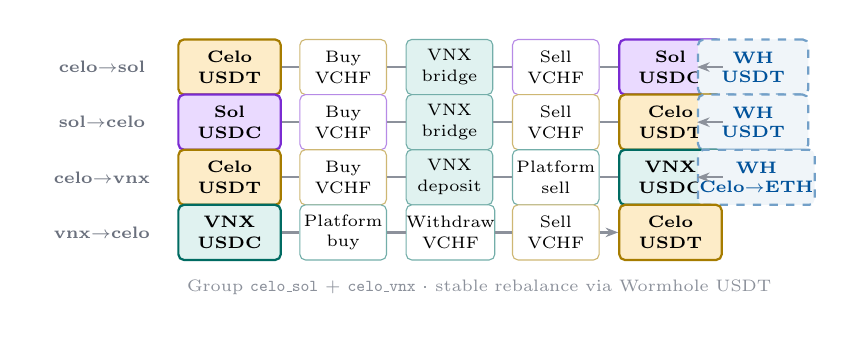
\begin{tikzpicture}[x=1mm,y=-1mm]
  \useasboundingbox (-19,0) rectangle (84,36);

  \node[rowlbl] at (-1,5) {celo$\rightarrow$sol};
  \node[hub=celostroke, fill=celofill, anchor=west] (c1s) at (\FxA,5) {Celo\\USDT};
  \node[act=celostroke, anchor=west] (c1b) at (\FxB,5) {Buy\\VCHF};
  \node[act=vnxstroke, fill=vnxfill, anchor=west] (c1v) at (\FxC,5) {VNX\\bridge};
  \node[act=solstroke, anchor=west] (c1x) at (\FxD,5) {Sell\\VCHF};
  \node[hub=solstroke, fill=solfill, anchor=west] (c1e) at (\FxE,5) {Sol\\USDC};
  \node[recon, anchor=west] (c1r) at (\FxR,5) {WH\\USDT};
  \draw[arr] (c1s)--(c1b)--(c1v)--(c1x)--(c1e)--(c1r);

  \node[rowlbl] at (-1,12) {sol$\rightarrow$celo};
  \node[hub=solstroke, fill=solfill, anchor=west] (c2s) at (\FxA,12) {Sol\\USDC};
  \node[act=solstroke, anchor=west] (c2b) at (\FxB,12) {Buy\\VCHF};
  \node[act=vnxstroke, fill=vnxfill, anchor=west] (c2v) at (\FxC,12) {VNX\\bridge};
  \node[act=celostroke, anchor=west] (c2x) at (\FxD,12) {Sell\\VCHF};
  \node[hub=celostroke, fill=celofill, anchor=west] (c2e) at (\FxE,12) {Celo\\USDT};
  \node[recon, anchor=west] (c2r) at (\FxR,12) {WH\\USDT};
  \draw[arr] (c2s)--(c2b)--(c2v)--(c2x)--(c2e)--(c2r);

  \node[rowlbl] at (-1,19) {celo$\rightarrow$vnx};
  \node[hub=celostroke, fill=celofill, anchor=west] (c3s) at (\FxA,19) {Celo\\USDT};
  \node[act=celostroke, anchor=west] (c3b) at (\FxB,19) {Buy\\VCHF};
  \node[act=vnxstroke, fill=vnxfill, anchor=west] (c3d) at (\FxC,19) {VNX\\deposit};
  \node[act=vnxstroke, anchor=west] (c3x) at (\FxD,19) {Platform\\sell};
  \node[hub=vnxstroke, fill=vnxfill, anchor=west] (c3e) at (\FxE,19) {VNX\\USDC};
  \node[recon, anchor=west] (c3r) at (\FxR,19) {WH\\Celo$\rightarrow$ETH};
  \draw[arr] (c3s)--(c3b)--(c3d)--(c3x)--(c3e)--(c3r);

  \node[rowlbl] at (-1,26) {vnx$\rightarrow$celo};
  \node[hub=vnxstroke, fill=vnxfill, anchor=west] (c4s) at (\FxA,26) {VNX\\USDC};
  \node[act=vnxstroke, anchor=west] (c4b) at (\FxB,26) {Platform\\buy};
  \node[act=vnxstroke, anchor=west] (c4w) at (\FxC,26) {Withdraw\\VCHF};
  \node[act=celostroke, anchor=west] (c4x) at (\FxD,26) {Sell\\VCHF};
  \node[hub=celostroke, fill=celofill, anchor=west] (c4e) at (\FxE,26) {Celo\\USDT};
  \draw[arr] (c4s)--(c4b)--(c4w)--(c4x)--(c4e);

  \node[anchor=west, font=\fontsize{6}{7.5}\selectfont, text=ink!50] at (0,33) {%
    Group \texttt{celo\_sol} + \texttt{celo\_vnx} · stable rebalance via Wormhole USDT};
\end{tikzpicture}}%
\vspace{0.5mm}
\end{minipage}}
\end{minipage}
&
\begin{minipage}[t]{\linewidth}
\noindent\fcolorbox{basestroke!30}{basefill!30}{%
\begin{minipage}{\dimexpr\linewidth-2\fboxsep-2\fboxrule\relax}
\vspace{0.5mm}
{\fontsize{8}{9.5}\selectfont\bfseries\color{basestroke} Base USDC hub --- 4 routes}\\[1mm]
\adjustbox{width=\linewidth, valign=t}{%
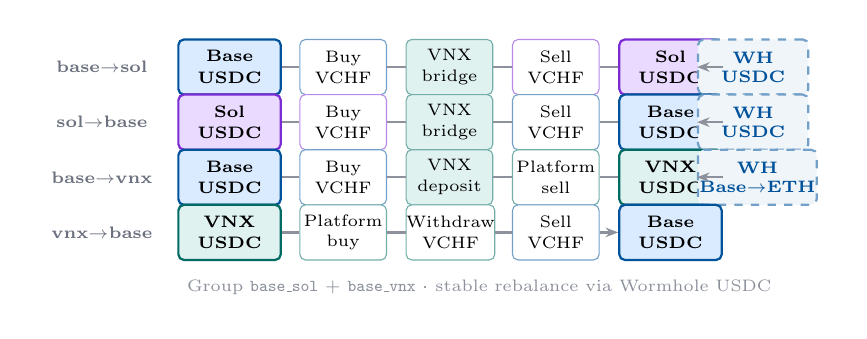
\begin{tikzpicture}[x=1mm,y=-1mm]
  \useasboundingbox (-19,0) rectangle (84,36);

  \node[rowlbl] at (-1,5) {base$\rightarrow$sol};
  \node[hub=basestroke, fill=basefill, anchor=west] (b1s) at (\FxA,5) {Base\\USDC};
  \node[act=basestroke, anchor=west] (b1b) at (\FxB,5) {Buy\\VCHF};
  \node[act=vnxstroke, fill=vnxfill, anchor=west] (b1v) at (\FxC,5) {VNX\\bridge};
  \node[act=solstroke, anchor=west] (b1x) at (\FxD,5) {Sell\\VCHF};
  \node[hub=solstroke, fill=solfill, anchor=west] (b1e) at (\FxE,5) {Sol\\USDC};
  \node[recon, anchor=west] (b1r) at (\FxR,5) {WH\\USDC};
  \draw[arr] (b1s)--(b1b)--(b1v)--(b1x)--(b1e)--(b1r);

  \node[rowlbl] at (-1,12) {sol$\rightarrow$base};
  \node[hub=solstroke, fill=solfill, anchor=west] (b2s) at (\FxA,12) {Sol\\USDC};
  \node[act=solstroke, anchor=west] (b2b) at (\FxB,12) {Buy\\VCHF};
  \node[act=vnxstroke, fill=vnxfill, anchor=west] (b2v) at (\FxC,12) {VNX\\bridge};
  \node[act=basestroke, anchor=west] (b2x) at (\FxD,12) {Sell\\VCHF};
  \node[hub=basestroke, fill=basefill, anchor=west] (b2e) at (\FxE,12) {Base\\USDC};
  \node[recon, anchor=west] (b2r) at (\FxR,12) {WH\\USDC};
  \draw[arr] (b2s)--(b2b)--(b2v)--(b2x)--(b2e)--(b2r);

  \node[rowlbl] at (-1,19) {base$\rightarrow$vnx};
  \node[hub=basestroke, fill=basefill, anchor=west] (b3s) at (\FxA,19) {Base\\USDC};
  \node[act=basestroke, anchor=west] (b3b) at (\FxB,19) {Buy\\VCHF};
  \node[act=vnxstroke, fill=vnxfill, anchor=west] (b3d) at (\FxC,19) {VNX\\deposit};
  \node[act=vnxstroke, anchor=west] (b3x) at (\FxD,19) {Platform\\sell};
  \node[hub=vnxstroke, fill=vnxfill, anchor=west] (b3e) at (\FxE,19) {VNX\\USDC};
  \node[recon, anchor=west] (b3r) at (\FxR,19) {WH\\Base$\rightarrow$ETH};
  \draw[arr] (b3s)--(b3b)--(b3d)--(b3x)--(b3e)--(b3r);

  \node[rowlbl] at (-1,26) {vnx$\rightarrow$base};
  \node[hub=vnxstroke, fill=vnxfill, anchor=west] (b4s) at (\FxA,26) {VNX\\USDC};
  \node[act=vnxstroke, anchor=west] (b4b) at (\FxB,26) {Platform\\buy};
  \node[act=vnxstroke, anchor=west] (b4w) at (\FxC,26) {Withdraw\\VCHF};
  \node[act=basestroke, anchor=west] (b4x) at (\FxD,26) {Sell\\VCHF};
  \node[hub=basestroke, fill=basefill, anchor=west] (b4e) at (\FxE,26) {Base\\USDC};
  \draw[arr] (b4s)--(b4b)--(b4w)--(b4x)--(b4e);

  \node[anchor=west, font=\fontsize{6}{7.5}\selectfont, text=ink!50] at (0,33) {%
    Group \texttt{base\_sol} + \texttt{base\_vnx} · stable rebalance via Wormhole USDC};
\end{tikzpicture}}%
\vspace{0.5mm}
\end{minipage}}
\end{minipage}
\\
\end{tabular}

\vspace{1mm}

% ── Sol ↔ VNX (shared) ──
\noindent\fcolorbox{vnxstroke!25}{vnxfill!40}{%
\begin{minipage}{\dimexpr\linewidth-2\fboxsep-2\fboxrule\relax}
\vspace{0.5mm}
{\fontsize{8}{9.5}\selectfont\bfseries\color{vnxstroke} Solana $\leftrightarrow$ VNX Platform --- 2 routes (group \texttt{vnx\_sol})}\\[1mm]
\adjustbox{width=0.98\linewidth, center}{%
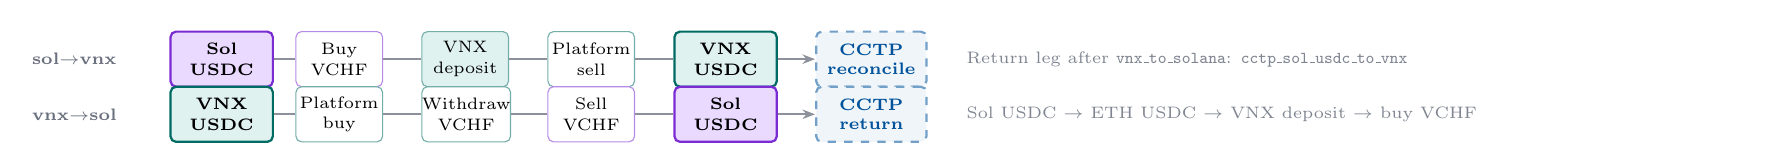
\begin{tikzpicture}[x=1mm,y=-1mm]
  \useasboundingbox (-18,0) rectangle (200,14);

  \node[rowlbl, minimum width=22mm] at (-1,4) {sol$\rightarrow$vnx};
  \node[hub=solstroke, fill=solfill, anchor=west] (s1s) at (0,4) {Sol\\USDC};
  \node[act=solstroke, anchor=west] (s1b) at (16,4) {Buy\\VCHF};
  \node[act=vnxstroke, fill=vnxfill, anchor=west] (s1d) at (32,4) {VNX\\deposit};
  \node[act=vnxstroke, anchor=west] (s1x) at (48,4) {Platform\\sell};
  \node[hub=vnxstroke, fill=vnxfill, anchor=west] (s1e) at (64,4) {VNX\\USDC};
  \node[recon, anchor=west] (s1r) at (82,4) {CCTP\\reconcile};
  \draw[arr] (s1s)--(s1b)--(s1d)--(s1x)--(s1e)--(s1r);

  \node[rowlbl, minimum width=22mm] at (-1,11) {vnx$\rightarrow$sol};
  \node[hub=vnxstroke, fill=vnxfill, anchor=west] (s2s) at (0,11) {VNX\\USDC};
  \node[act=vnxstroke, anchor=west] (s2b) at (16,11) {Platform\\buy};
  \node[act=vnxstroke, anchor=west] (s2w) at (32,11) {Withdraw\\VCHF};
  \node[act=solstroke, anchor=west] (s2x) at (48,11) {Sell\\VCHF};
  \node[hub=solstroke, fill=solfill, anchor=west] (s2e) at (64,11) {Sol\\USDC};
  \node[recon, anchor=west] (s2r) at (82,11) {CCTP\\return};
  \draw[arr] (s2s)--(s2b)--(s2w)--(s2x)--(s2e)--(s2r);

  \node[anchor=west, font=\fontsize{6}{7.5}\selectfont, text=ink!55] at (100,4) {%
    Return leg after \texttt{vnx\_to\_solana}: \texttt{cctp\_sol\_usdc\_to\_vnx}};
  \node[anchor=west, font=\fontsize{6}{7.5}\selectfont, text=ink!55] at (100,11) {%
    Sol USDC $\rightarrow$ ETH USDC $\rightarrow$ VNX deposit $\rightarrow$ buy VCHF};
\end{tikzpicture}}%
\vspace{0.5mm}
\end{minipage}}

\vspace{1mm}
\noindent\rule{\linewidth}{0.3pt}
\vspace{0.5mm}

% ── Footer ──
\noindent
\begin{tabular}{@{}>{\raggedright\arraybackslash}p{0.64\linewidth}@{\hspace{0.02\linewidth}}>{\raggedright\arraybackslash}p{0.33\linewidth}@{}}
\begin{minipage}[t]{\linewidth}
  {\fontsize{7}{8.5}\selectfont
  \textbf{Source:} \texttt{src/scanner/routes.py} · \textbf{Token:} VCHF · \textbf{Pair:} \texttt{VCHF/USDC}\\
  \textbf{No direct Celo$\leftrightarrow$Base} --- cross via Solana or VNX platform · ETH hub = USDC settlement only}
\end{minipage}
&
\begin{minipage}[t]{\linewidth}
  \raggedleft
  {\fontsize{7}{8.5}\selectfont
  \textbf{Build:} \texttt{python scripts/generate\_routes\_pdf.py --executive}\\
  \textbf{Matrix:} \texttt{scripts/execute\_route\_matrix.py}}
\end{minipage}
\\
\end{tabular}

\end{document}
